
\section*{Logische Verknüpfungen}

Für N eingänge hat man 2$^{N}$ Eingangskombinationen.

Elementare Logische Funktionen: NOT, AND, OR, NAND, NOR, XOR, XNOR
\begin{verse}
\begin{tabular}{|c||c||c||c||c||c||c||c||c||c||c}
\hline 
\multicolumn{11}{|c}{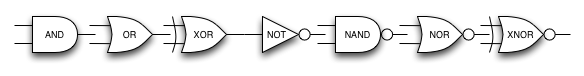
\includegraphics[height=1cm]{DT/img/baust}}\tabularnewline
\hline 
\end{tabular}%
\begin{tabular}{|c||c||c||c||c||c||c||c||c||c||c}
\hline 
\multicolumn{11}{|c}{\includegraphics[height=1cm]{\string"DT/2013-06-26 14.42.37\string".jpg}}\tabularnewline
\hline 
\end{tabular}
\end{verse}

\section*{Zahlensysteme}

\begin{tabular}{cc}
\begin{tabular}{|c|c|c|}
\hline 
Dezimal & Binary & Hex\tabularnewline
\hline 
\hline 
0 & 0000 & 0\tabularnewline
\hline 
1 & 0001 & 1\tabularnewline
\hline 
2 & 0010 & 2\tabularnewline
\hline 
3 & 0011 & 3\tabularnewline
\hline 
4 & 0100 & 4\tabularnewline
\hline 
5 & 0101 & 5\tabularnewline
\hline 
6 & 0110 & 6\tabularnewline
\hline 
7 & 0111 & 7\tabularnewline
\hline 
8 & 1000 & 8\tabularnewline
\hline 
9 & 1001 & 9\tabularnewline
\hline 
10 & 1010 & A\tabularnewline
\hline 
11 & 1011 & B\tabularnewline
\hline 
12 & 1100 & C\tabularnewline
\hline 
13 & 1101 & D\tabularnewline
\hline 
14 & 1110 & E\tabularnewline
\hline 
15 & 1111 & F\tabularnewline
\hline 
\end{tabular} & %
\begin{tabular}{cll}
LSB: & Least Significant Bit - z.B.: $2^{0}$ & \tabularnewline
Nibble: & Gruppe von 4 Bit & \tabularnewline
Byte: & Gruppe von 8 Bit (2Nibble) & \tabularnewline
Word: & Gruppe von mehr als 8 Bit (Meisstens 16Bit) & \tabularnewline
DWord: & Double Word: oft eine Gruppe von 32 Bit & \tabularnewline
 &  & \tabularnewline
Bsp: & 1011 1100 0010 (BIN) = BC2 (HEX) & \tabularnewline
 & 101 111 000 010 (BIN) = 5702 (OCTAL) & \tabularnewline
 &  & \tabularnewline
 & Divisionsmethode: & \tabularnewline
 & 47 b10 = 101111 b2 & \tabularnewline
\cline{2-3} 
 & 47 : 2 = 23 r1 & LSB\tabularnewline
 & 23 : 2 = 11 r1 & \tabularnewline
 & 11 : 2 = 5 r1 & \tabularnewline
 & 5 : 2 = 2 r1 & \tabularnewline
 & 2 : 2 = 1 r0 & \tabularnewline
 & 1 : 2 = 0 r1 & MSB\tabularnewline
\end{tabular}\tabularnewline
\end{tabular}


\section*{Schaltalgebra}

\begin{tabular}{|c|c|c|}
\hline 
Funktion & mit NOR ausgedrückt: & mit NAND ausgedrückt:\tabularnewline
\hline 
\hline 
NOT & \includegraphics[height=0.35cm]{DT/img/no3} & !(X \& X)\tabularnewline
\hline 
OR & \includegraphics[height=0.5cm]{DT/img/nor2} & !( !(X\&X) \& !(Y\&Y) )\tabularnewline
\hline 
AND & \includegraphics[height=0.5cm]{DT/img/nor1} & !( !(X \& Y) \& !(X \& Y) )\tabularnewline
\hline 
NOR & trivial & !( !( !(X\&X) \& !(Y\&Y) ) \& !( !(X\&X) \& !(Y\&Y) ) )\tabularnewline
\hline 
XOR & {[}(AnorA)nor(BnorB){]}nor(AnorB) & !( !( X \& !(X\&Y) ) \& !( Y \& !(X\&Y) ) )\tabularnewline
\hline 
NAND & AND with NOT & trivial\tabularnewline
\hline 
\end{tabular}


\subsection*{Vereinfachungen}
\begin{itemize}
\item Kommutativgesetze

\begin{itemize}
\item A \& B = B \& A 
\item A \# B = B \# A 
\end{itemize}
\item Assoziativgesetze 

\begin{itemize}
\item (A \& B) \& C = A \& (B \& C) 
\item (A \# B) \# C = A \# (B \# C) 
\end{itemize}
\item Distributivgesetze 

\begin{itemize}
\item (A \# B) \& C = (A \& C) \# (B \& C) 
\item (A \& B) \# C = (A \# C) \& (B \# C)
\end{itemize}
\item Vereinfachungen

\begin{itemize}
\item A \# (A \& B) = A
\item A \& (A \# B) = A
\item A \# (!A \& B) = A \# B
\item A \& (!A \# B) = A \& B
\end{itemize}
\end{itemize}

\subsection*{Disjunktive Normalform}
\begin{itemize}
\item OR Verknüpfung von AND Blöcken für K=1
\item Jeder AND-Block ist ein MINTERM
\item Die DNF K ist eine OR-Verknüpfung aller guten MINTERME (gut = Wahrheitstabelle
1)
\end{itemize}
Für die Darstellung mit NAND anstelle von OR:

Das DeMorgan Theorem anwenden: $K=!(!K)$ und dann weiter vereinfachen.


\subsection*{Konjunktive Normalform}
\begin{itemize}
\item AND Verknüpfung von OR Blöcken
\item Herstellen durch DNF von K=0, dann DeMorgan Theorem anwenden
\item Jeder OR-Block ist ein schlechter MAXTERM, der einer Zeile in der
Wahrheitstabelle entspricht, negiert wenn in der Wahrheitstabelle
=1, direkt falls WT=0.
\item guter Maxterm ist negierter Block von schlechten Maxtermen\end{itemize}
\begin{verse}
Multiplexer:

Art von Drehschalter, umschalten zwischen verschiedenen Eingängen
\end{verse}

\section*{Vorzeichenlose und Vorzeichenbehaftete Zahlen}

\begin{tabular}{|c|c|c|c|c|c|c|c|}
\hline 
Typ & min & -2 & -1 & 0 & 1 & 2 & max\tabularnewline
\hline 
\hline 
Unsigned & - & - & - & 0000 & 0001 & 0010 & 1111 (15)\tabularnewline
\hline 
One's Complement & 1000 (-7) & 1101 & 1110 & 0000, 1111 & 0001 & 0010 & 0111 (7)\tabularnewline
\hline 
Two's Complement & 1000 (-8) & 1110 & 1111 & 0000 & 0001 & 0010 & 0111 (7)\tabularnewline
\hline 
Sign Magnitude & 1111 (-7) & 1010 & 1001 & 0000, 1000 & 0001 & 0010 & 0111 (7)\tabularnewline
\hline 
\end{tabular}

CF: Carry Flag: Übertrag beim Addieren

OF: Overflow Flag: Über oder Unterlaufen


\subsection*{Addition und Subtraktion}

\begin{tabular}{|c|c|c|c|c|c|c|c|}
\hline 
\multicolumn{2}{|c|}{Operanden} & \multicolumn{3}{c|}{Addition} & \multicolumn{3}{c|}{Subtraktion}\tabularnewline
\hline 
\hline 
op1 & op2 & op1+op2 & carry & overflow & op1-op2 & borrow & overflow\tabularnewline
\hline 
6C & 97 & 03 & 1 & 0 &  &  & 1\tabularnewline
\hline 
76 & 33 & A9 & 1 & 1 & 43 & 0 & 0\tabularnewline
\hline 
\end{tabular}

Addition: %
\begin{tabular}{|c|c|c|c|c|c|c|c|}
\hline 
0 & 1 & 1 & 0 & 1 & 1 & 0 & 0\tabularnewline
\hline 
1 & 0 & 0 & 1 & 0 & 1 & 1 & 1\tabularnewline
\hline 
\hline 
\textcolor{red}{1} & 1 & 1 & 1 & 1 & - & - & -\tabularnewline
\hline 
\hline 
\textbf{0} & \textbf{0} & \textbf{0} & \textbf{0} & \textbf{0} & \textbf{0} & \textbf{1} & \textbf{1}\tabularnewline
\hline 
\end{tabular}%
\begin{tabular}{|c|c|}
\hline 
\textbf{Carry} & \textbf{Overflow}\tabularnewline
\hline 
\hline 
1 & 1xor1= 0\tabularnewline
\hline 
\end{tabular}%
\begin{tabular}{|c|c|c|c|c|c|c|c|}
\hline 
0 & 1 & 1 & 1 & 0 & 1 & 1 & 0\tabularnewline
\hline 
0 & 0 & 1 & 1 & 0 & 0 & 1 & 1\tabularnewline
\hline 
\hline 
\textcolor{red}{1} & 1 & 1 & - & 1 & 1 & - & -\tabularnewline
\hline 
\hline 
\textbf{1} & \textbf{0} & \textbf{1} & \textbf{0} & \textbf{1} & \textbf{0} & \textbf{0} & \textbf{1}\tabularnewline
\hline 
\end{tabular}%
\begin{tabular}{|c|c|}
\hline 
\textbf{Carry} & \textbf{Overflow}\tabularnewline
\hline 
\hline 
0 & 0xor1= 1\tabularnewline
\hline 
\end{tabular}

Subtraktion: %
\begin{tabular}{|c|c|c|c|c|c|c|c|}
\hline 
0 & 1 & 1 & 0 & 1 & 1 & 0 & 0\tabularnewline
\hline 
1 & 0 & 0 & 1 & 0 & 1 & 1 & 1\tabularnewline
\hline 
\hline 
\textcolor{red}{0} & 0 & 1 & 0 & 1 & 1 & 1 & 0\tabularnewline
\hline 
\hline 
\textbf{1} & \textbf{1} & \textbf{0} & \textbf{1} & \textbf{0} & \textbf{1} & \textbf{0} & \textbf{1}\tabularnewline
\hline 
\end{tabular}%
\begin{tabular}{|c|c|}
\hline 
\textbf{C/Borrow} & \textbf{Overflow}\tabularnewline
\hline 
\hline 
0 & 0xor1= 1\tabularnewline
\hline 
\end{tabular}%
\begin{tabular}{|c|c|c|c|c|c|c|c|}
\hline 
0 & 1 & 1 & 1 & 0 & 1 & 1 & 0\tabularnewline
\hline 
0 & 0 & 1 & 1 & 0 & 0 & 1 & 1\tabularnewline
\hline 
\hline 
\textcolor{red}{0} & 0 & 0 & 0 & 0 & 1 & 1 & 0\tabularnewline
\hline 
\hline 
\textbf{0} & \textbf{1} & \textbf{0} & \textbf{0} & \textbf{0} & \textbf{0} & \textbf{1} & \textbf{1}\tabularnewline
\hline 
\end{tabular}%
\begin{tabular}{|c|c|}
\hline 
\textbf{C/Borrow} & \textbf{Overflow}\tabularnewline
\hline 
\hline 
0 & 0xor0= 0\tabularnewline
\hline 
\end{tabular}
